\section{Experiment 9K: blind confirmation of distributed personalization}
\label{sec:experiment9k}

\paragraph{Frozen protocol.}
Experiment 9K evaluates the complete Experiment 9J protocol on the ten seeds
206--215 that were reserved before 9J was executed. A machine-checked freeze
requires every inherited data volume, algorithmic setting, model-order
candidate, communication round, participation rate, progressive rank, and
nonlinear scenario to equal 9J. No development result or confirmation result
is used for tuning.

Five primary gates were declared before execution: Fed100 must degrade by less
than 0.1\% relative to the established Central implementation; Fed50 and Fed20
must degrade by less than 1\% and 2\%, respectively; Fed20 must beat Local at
the 0.75~s cold-start budget; and every nonlinear closed-loop evaluation must
remain feasible. The 1.25~s Fed20--Local comparison was deliberately excluded
from the positive gate because Experiment 9J predicted parity after Local
identification acquired sufficient data.

\begin{table}[htbp]
\centering
\caption{Experiment 9K blind-confirmation tracking RMSE. Percentages compare
with the Central implementation.}
\label{tab:experiment9k-results}
\begin{tabular}{lrrrr}
\toprule
Method & \multicolumn{2}{c}{0.75 s} & \multicolumn{2}{c}{1.25 s}\\
 & RMSE & vs. Central & RMSE & vs. Central\\
\midrule
Local   & 0.012714 & +18.47\% & 0.007557 & +0.36\%\\
Central & 0.010731 & 0.00\%   & 0.007530 & 0.00\%\\
Fed100  & 0.010762 & +0.28\%  & 0.007531 & +0.02\%\\
Fed50   & 0.010648 & -0.77\%  & 0.007548 & +0.25\%\\
Fed20   & 0.010518 & -1.99\%  & 0.007562 & +0.42\%\\
\bottomrule
\end{tabular}
\end{table}

\begin{figure}[htbp]
\centering
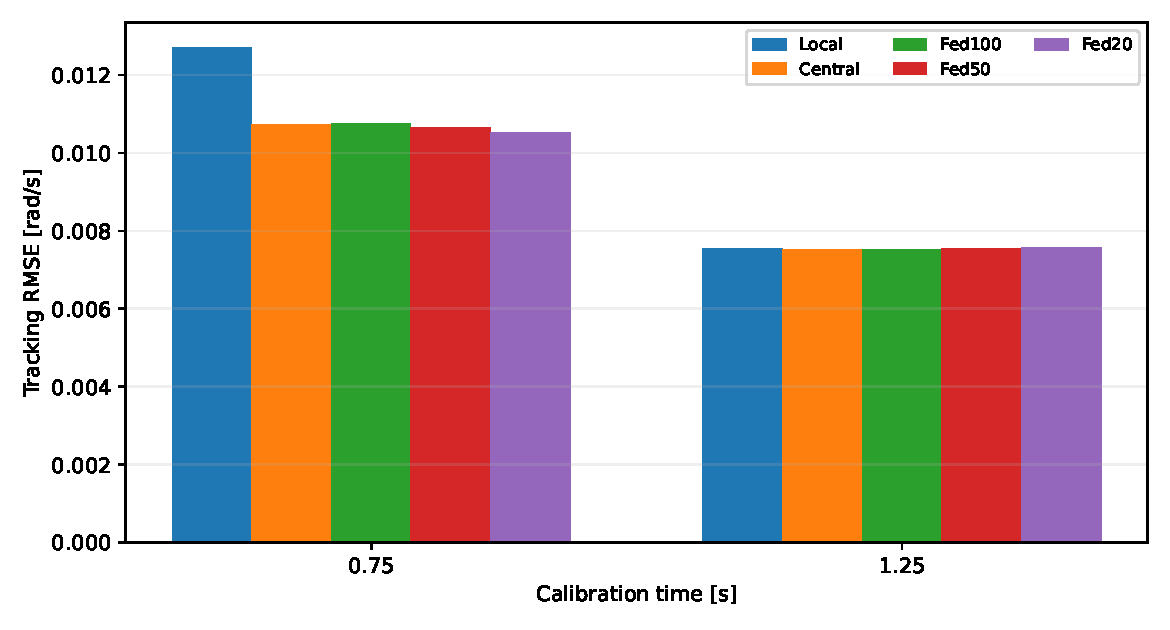
\includegraphics[width=0.84\linewidth]{../results/figures/experiment_9k_blind_confirmation.pdf}
\caption{Blind confirmation preserves the large cold-start benefit and the
later convergence toward Local performance.}
\label{fig:experiment9k}
\end{figure}

\paragraph{Gate outcome.}
Four of the five primary gates pass. Fed50 and Fed20 stay below their permitted
degradation, Fed20 beats Local at 0.75~s, and all 10800 nonlinear evaluations
remain feasible. The strict Fed100 equivalence gate fails: its aggregate
tracking is 0.281\% worse than Central at 0.75~s, exceeding the predeclared
0.1\% tolerance. At 1.25~s the difference is 0.020\%. This threshold is not
changed after observing the data.

The failed gate separates two notions that were nearly indistinguishable in
9J. A deterministic rerun of the federated aggregation reproduces its selected
group count, means, and covariances below $10^{-12}$ and therefore passes the
internal implementation check. Central and Fed100, however, use different
mixture-fitting implementations and need not produce exactly the same finite-
sample optimum. The confirmation shows that they are control-equivalent to
well below 1\%, but it does not support a 0.1\% numerical-equivalence claim.

\paragraph{Confirmed scientific result.}
At 0.75~s, Fed20 improves aggregate tracking over Local by 17.27\%; the mean
paired fleet improvement is 16.90\%, and Fed20 wins nine of ten fleet-wise
comparisons. Fed50 improves the aggregate result by 16.24\% and also wins nine
of ten fleets. The effect is therefore smaller than the 21.09\% development
estimate but remains large and consistent on untouched fleets.

At 1.25~s, Fed20 is 0.06\% worse than Local and wins five of ten fleets; Fed50
is 0.11\% better and wins seven. This confirms the predicted transition to
parity rather than continued federated superiority. The evidence supports a
specific deployment claim: a mature fleet representation protects a new client
during cold start, while sufficiently informative local identification catches
up.

Fed100 selects three groups on every fleet with mean ARI 0.997. Fed50 and Fed20
obtain mean ARI 0.937 and 0.917; occasional under- or over-partitioning does not
destroy the control result. All 2400 fits converge. Together with the 9J
development results, the confirmation rules out a favorable-seed explanation
for the main cold-start finding.

\paragraph{Decision.}
Experiment 9K confirms the paper's main personalized-FL claim but narrows the
implementation statement. The manuscript should claim sub-percent agreement
between full-participation federated and Central learning, not exact equivalence.
The failed 0.1\% gate should be reported transparently. The next robustness
question is nonrandom availability: random partial participation retains almost
complete client coverage and approximately balanced groups, whereas a deployed
fleet may systematically omit a family or operating region.

\paragraph{Reproducibility.}
The frozen configuration and gates are in
\path{code/config/experiment_9k.json}. The confirmation driver is
\path{code/experiments/experiment_9k_blind_confirmation.py}; it refuses to run
if inherited 9J settings or the reserved seed set differ. Aggregate, seed-level,
communication, gate, and provenance records are stored under
\path{results/tables}.
